\documentclass[aspectratio=169]{beamer}

\usepackage[T1]{fontenc}
\usepackage[utf8]{inputenc}
\usepackage{lmodern}
\usepackage{microtype}
\usepackage{xcolor}
\usepackage{tikz}
\usetikzlibrary{positioning, arrows.meta}
\usepackage{booktabs}
\usepackage{fontawesome5}

\definecolor{wurgreen}{HTML}{34B233}
\definecolor{darkgreen}{HTML}{1F6B1E}
\definecolor{darknavy}{HTML}{1A1A2E}
\definecolor{midgray}{HTML}{6B7280}
\definecolor{lightgray}{HTML}{F3F4F6}
\definecolor{lightgreen}{HTML}{E8F7E8}
\definecolor{bodytext}{HTML}{1F2937}
\definecolor{warnred}{HTML}{FEE2E2}
\definecolor{warnborder}{HTML}{EF4444}

\usetheme{default}
\usecolortheme{default}
\usefonttheme{professionalfonts}
\setbeamertemplate{navigation symbols}{}
\setbeamertemplate{itemize items}{\textcolor{wurgreen}{\textbullet}}
\setbeamertemplate{itemize subitem}{\textcolor{midgray}{--}}
\setbeamercolor{frametitle}{fg=white, bg=darknavy}
\setbeamerfont{frametitle}{size=\large, series=\bfseries}
\setbeamertemplate{frametitle}{%
  \begin{beamercolorbox}[wd=\paperwidth, ht=1.1cm, dp=0.2cm, leftskip=0.6cm]{frametitle}
    \usebeamerfont{frametitle}\insertframetitle
  \end{beamercolorbox}}
\setbeamercolor{background canvas}{bg=white}
\setbeamercolor{normal text}{fg=bodytext}
\setbeamertemplate{footline}{%
  \begin{beamercolorbox}[wd=\paperwidth, ht=0.4cm, dp=0.15cm]{footline}
    \hspace{0.5cm}\textcolor{midgray}{\tiny Bags, Vectors \& Transformers · Wageningen University \& Research}%
    \hfill\textcolor{midgray}{\tiny \insertframenumber}\hspace{0.4cm}
  \end{beamercolorbox}}

\begin{document}

% ── TITLE SLIDE ──────────────────────────────────────────────────────────────
{
\setbeamertemplate{footline}{}
\begin{frame}[plain]
  \begin{tikzpicture}[remember picture, overlay]
    \fill[darknavy] (current page.south west) rectangle (current page.north east);
    \fill[wurgreen] (current page.south west) rectangle
      ([xshift=0.45cm]current page.north west);
    \node[anchor=west, text=white, font=\huge\bfseries, text width=13cm]
      at ([xshift=1.1cm, yshift=1.2cm]current page.west)
      {Bags, Vectors \& Transformers};
    \node[anchor=west, text=wurgreen, font=\large, text width=12cm]
      at ([xshift=1.1cm, yshift=0.05cm]current page.west)
      {Foundations of Word Embeddings · Day 2, Part 1};
    \node[anchor=west, text=midgray, font=\small, text width=12cm]
      at ([xshift=1.1cm, yshift=-1.5cm]current page.west)
      {Denise J. Roth, PhD Candidate\\
       Strategic Communication Group · Wageningen University \& Research};
  \end{tikzpicture}
\end{frame}
}

% ── SLIDE 1: Welcome back / recap ────────────────────────────────────────────
\begin{frame}{Welcome Back --- Where We Left Off}
\vspace{0.2cm}
{\small Yesterday we built the \textbf{classic toolkit} for turning text into data. A quick recap:}

\medskip
\begin{columns}[T]
  \column{0.48\textwidth}
  \vspace{0pt}
  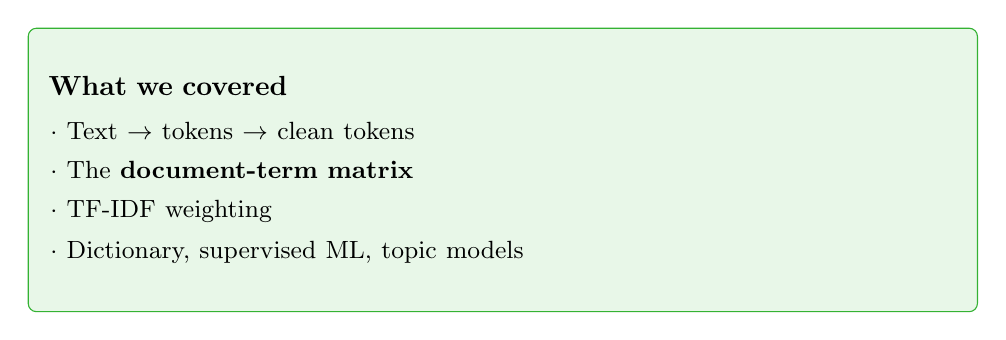
\begin{tikzpicture}
    \node[fill=lightgreen, draw=wurgreen, rounded corners=3pt,
          inner xsep=8pt, inner ysep=8pt, text width=\columnwidth-18pt, minimum height=3.6cm]{%
      \textbf{What we covered}\\[5pt]
      {\small
      $\cdot$ Text $\rightarrow$ tokens $\rightarrow$ clean tokens\\[3pt]
      $\cdot$ The \textbf{document-term matrix}\\[3pt]
      $\cdot$ TF-IDF weighting\\[3pt]
      $\cdot$ Dictionary, supervised ML, topic models}};
  \end{tikzpicture}

  \column{0.48\textwidth}
  \vspace{0pt}
  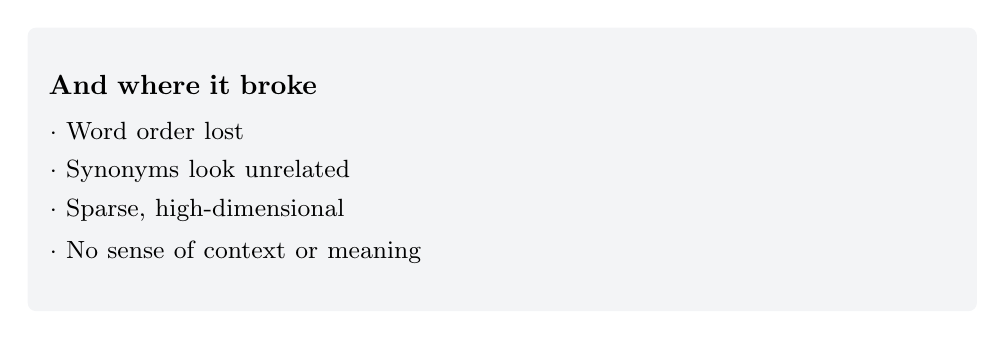
\begin{tikzpicture}
    \node[fill=lightgray, rounded corners=3pt,
          inner xsep=8pt, inner ysep=8pt, text width=\columnwidth-18pt, minimum height=3.6cm]{%
      \textbf{And where it broke}\\[5pt]
      {\small
      $\cdot$ Word order lost\\[3pt]
      $\cdot$ Synonyms look unrelated\\[3pt]
      $\cdot$ Sparse, high-dimensional\\[3pt]
      $\cdot$ No sense of context or meaning}};
  \end{tikzpicture}
\end{columns}

\medskip
{\small\textcolor{midgray}{\textit{Today we address that last column --- starting with the idea of representing
meaning itself.}}}
\end{frame}

% ── SLIDE 2: Questions ───────────────────────────────────────────────────────
\begin{frame}{Before We Dive In}
\vspace{1.2cm}
\begin{center}
{\Large\bfseries Any questions from yesterday? \faComments}
\end{center}

\vspace{0.8cm}
\begin{center}
\begin{minipage}{0.8\textwidth}
{\small\textcolor{midgray}{\centering
Anything from the notebooks, the document-term matrix, the three approaches,
or the limitations we saw? \\[6pt]
Now is a good moment --- today builds directly on these ideas.}}
\end{minipage}
\end{center}
\end{frame}

% ── SLIDE 3: The core problem restated ───────────────────────────────────────
\begin{frame}{The Problem We Want to Solve}
\vspace{0.2cm}
{\small Bag-of-words treats every word as an \textbf{isolated symbol}. ``happy'', ``joyful'',
and ``concrete'' are just three different columns --- equally unrelated to one another.}

\bigskip
{\small What we \emph{want} is a representation where a word's \textbf{meaning} is captured,
so that words with similar meanings have similar representations. The question is:}

\medskip
\begin{center}
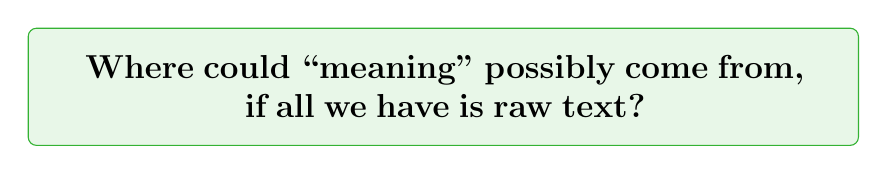
\begin{tikzpicture}
  \node[fill=lightgreen, draw=wurgreen, rounded corners=3pt,
        inner xsep=12pt, inner ysep=10pt, text width=0.8\textwidth]{%
    {\centering\large\textbf{Where could ``meaning'' possibly come from,\\
    if all we have is raw text?}\par}};
\end{tikzpicture}
\end{center}

\medskip
{\small\textcolor{midgray}{\textit{The answer is one of the most influential ideas in
language science.}}}
\end{frame}

% ── SLIDE 4: Distributional hypothesis ───────────────────────────────────────
\begin{frame}{The Distributional Hypothesis}
\vspace{0.2cm}
\begin{center}
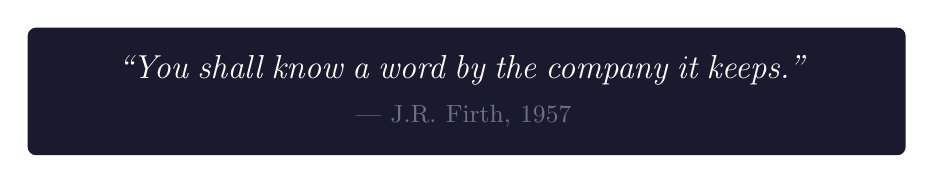
\begin{tikzpicture}
  \node[fill=darknavy, rounded corners=3pt,
        inner xsep=12pt, inner ysep=10pt, text width=0.85\textwidth]{%
    {\centering\textcolor{white}{\large\textit{``You shall know a word by the company it keeps.''}}\\[4pt]
    \textcolor{midgray}{\small --- J.R. Firth, 1957}\par}};
\end{tikzpicture}
\end{center}

\bigskip
{\small The \textbf{distributional hypothesis} is the idea that words appearing in
\textbf{similar contexts} tend to have \textbf{similar meanings}. Meaning is not an intrinsic
label --- it can be inferred from \textbf{patterns of use}.}

\medskip
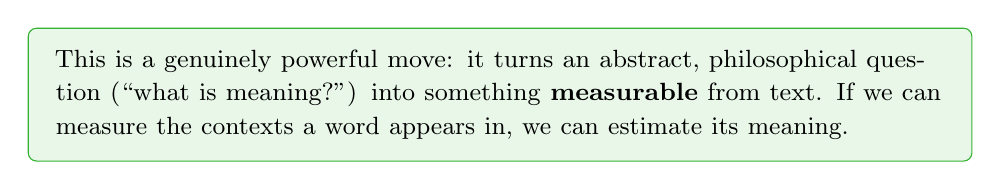
\begin{tikzpicture}
  \node[fill=lightgreen, draw=wurgreen, rounded corners=3pt,
        inner xsep=10pt, inner ysep=8pt, text width=\textwidth-24pt]{%
    {\small This is a genuinely powerful move: it turns an abstract, philosophical question
    (``what is meaning?'') into something \textbf{measurable} from text. If we can measure
    the contexts a word appears in, we can estimate its meaning.}};
\end{tikzpicture}
\end{frame}

% ── SLIDE 5: An intuitive example ────────────────────────────────────────────
\begin{frame}{An Intuition: Guess the Word}
\vspace{0.2cm}
{\small Suppose you keep seeing an unfamiliar word --- let's call it \textbf{``wug''} ---
in sentences like these:}

\medskip
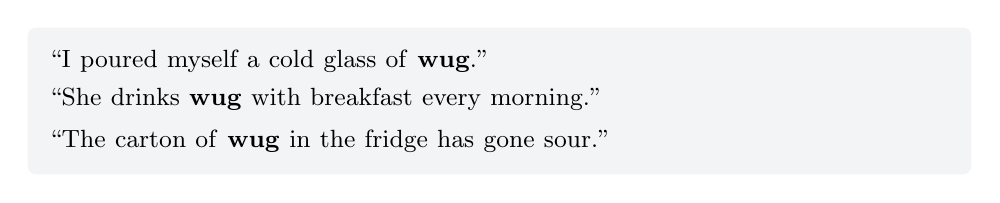
\begin{tikzpicture}
  \node[fill=lightgray, rounded corners=3pt,
        inner xsep=10pt, inner ysep=8pt, text width=\textwidth-24pt]{%
    {\small
    ``I poured myself a cold glass of \textbf{wug}.''\\[3pt]
    ``She drinks \textbf{wug} with breakfast every morning.''\\[3pt]
    ``The carton of \textbf{wug} in the fridge has gone sour.''}};
\end{tikzpicture}

\bigskip
{\small You have never been told what ``wug'' means --- but you already have a strong guess.
Something like \textbf{milk}. How? You inferred it \textbf{entirely from context}: the words
that surround it (glass, drinks, breakfast, carton, fridge, sour).}

\medskip
{\small\textcolor{midgray}{\textit{That is the distributional hypothesis at work --- and it is
exactly what embedding methods automate over billions of sentences.}}}
\end{frame}

% ── SLIDE 6: From contexts to vectors ────────────────────────────────────────
\begin{frame}{From Contexts to Vectors}
\vspace{0.2cm}
{\small If meaning comes from context, we can represent each word by \textbf{the company it
keeps} --- as a \textbf{vector of numbers}. Words used in similar contexts get similar vectors.}

\bigskip
\begin{columns}[T]
  \column{0.48\textwidth}
  \vspace{0pt}
  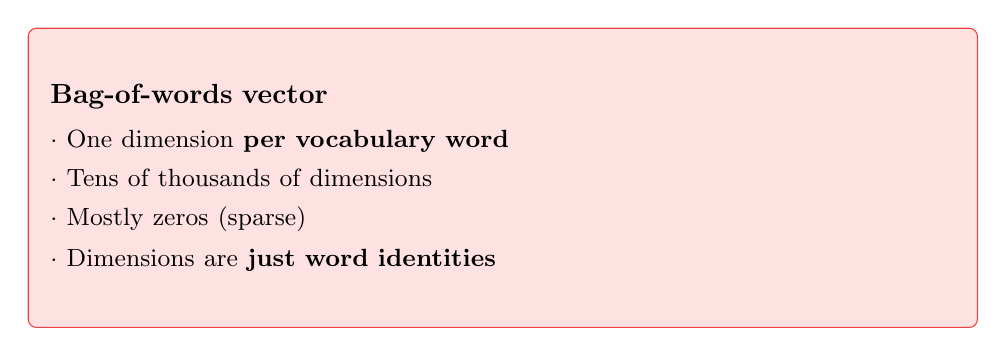
\begin{tikzpicture}
    \node[fill=warnred, draw=warnborder, rounded corners=3pt,
          inner xsep=8pt, inner ysep=8pt, text width=\columnwidth-18pt, minimum height=3.8cm]{%
      \textbf{Bag-of-words vector}\\[5pt]
      {\small
      $\cdot$ One dimension \textbf{per vocabulary word}\\[3pt]
      $\cdot$ Tens of thousands of dimensions\\[3pt]
      $\cdot$ Mostly zeros (sparse)\\[3pt]
      $\cdot$ Dimensions are \textbf{just word identities}}};
  \end{tikzpicture}

  \column{0.48\textwidth}
  \vspace{0pt}
  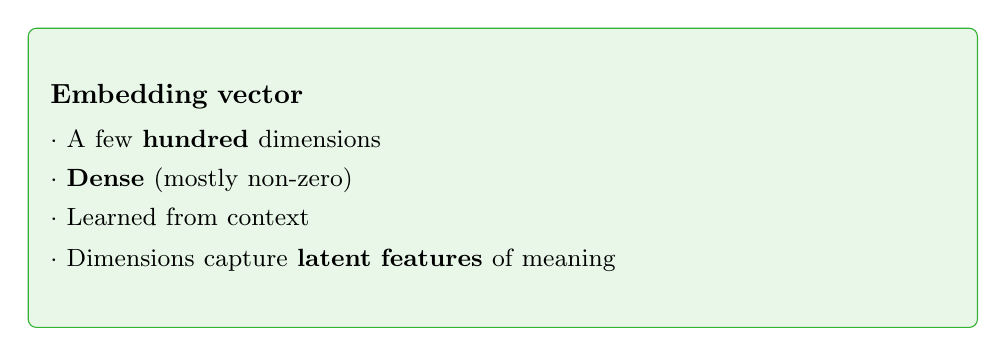
\begin{tikzpicture}
    \node[fill=lightgreen, draw=wurgreen, rounded corners=3pt,
          inner xsep=8pt, inner ysep=8pt, text width=\columnwidth-18pt, minimum height=3.8cm]{%
      \textbf{Embedding vector}\\[5pt]
      {\small
      $\cdot$ A few \textbf{hundred} dimensions\\[3pt]
      $\cdot$ \textbf{Dense} (mostly non-zero)\\[3pt]
      $\cdot$ Learned from context\\[3pt]
      $\cdot$ Dimensions capture \textbf{latent features} of meaning}};
  \end{tikzpicture}
\end{columns}

\medskip
{\small\textcolor{midgray}{\textit{We call these dense vectors \textbf{word embeddings}: each
word is ``embedded'' as a point in a shared meaning-space.}}}
\end{frame}

% ── SLIDE 7: The meaning space ───────────────────────────────────────────────
\begin{frame}{Words as Points in Space}
\vspace{0.1cm}
{\small The key payoff: in embedding space, \textbf{distance means something}. Words with
similar meanings sit \textbf{close together}; unrelated words sit far apart.}

\smallskip
\begin{center}
\begin{tikzpicture}[scale=0.72]
  % axes
  \draw[->, midgray] (0,0) -- (9,0);
  \draw[->, midgray] (0,0) -- (0,5);
  % cluster 1: emotions
  \fill[wurgreen] (1.5,3.8) circle (2pt) node[right, font=\scriptsize] {happy};
  \fill[wurgreen] (2.1,4.1) circle (2pt) node[right, font=\scriptsize] {joyful};
  \fill[wurgreen] (1.8,3.3) circle (2pt) node[right, font=\scriptsize] {cheerful};
  \draw[wurgreen, dashed, opacity=0.5] (1.8,3.7) circle (0.9);
  % cluster 2: animals
  \fill[darknavy] (6.5,1.2) circle (2pt) node[right, font=\scriptsize] {dog};
  \fill[darknavy] (7.1,1.6) circle (2pt) node[right, font=\scriptsize] {cat};
  \fill[darknavy] (6.8,0.7) circle (2pt) node[right, font=\scriptsize] {rabbit};
  \draw[darknavy, dashed, opacity=0.5] (6.8,1.15) circle (0.9);
\end{tikzpicture}
\end{center}

\smallskip
{\small ``happy'', ``joyful'', ``cheerful'' cluster together; ``dog'', ``cat'', ``rabbit''
form a separate cluster. The model was never \emph{told} these groupings --- it discovered
them from context. \textcolor{midgray}{\textit{(A 2-D sketch; real embeddings have hundreds
of dimensions.)}}}
\end{frame}

% ── SLIDE 8: Analogies ───────────────────────────────────────────────────────
\begin{frame}{A Famous Consequence: Analogies}
\vspace{0.2cm}
{\small Because meaning is encoded geometrically, \textbf{directions} in the space can carry
meaning too. The classic example:}

\bigskip
\begin{center}

\begin{tikzpicture}
  \node[fill=lightgreen, draw=wurgreen, rounded corners=3pt,
        inner xsep=12pt, inner ysep=10pt, text width=0.75\textwidth]{%
    {\centering\large
    \textbf{king} $-$ \textbf{man} $+$ \textbf{woman} $\approx$ \textbf{queen}\par}};
\end{tikzpicture}
\end{center}

\bigskip
{\small The vector that takes you from ``man'' to ``woman'' is roughly the \emph{same} vector
that takes you from ``king'' to ``queen''. A ``gender direction'' emerges in the space, along
with directions for tense, plurality, even country-to-capital.}

\medskip
{\small\textcolor{midgray}{\textit{This was the result that made embeddings famous around 2013
--- and it falls out of the distributional hypothesis, no hand-coding required.}}}
\end{frame}

% ── SLIDE 9: Two flavors preview ─────────────────────────────────────────────
\begin{frame}{Two Flavors of Embeddings}
\vspace{0.3cm}
\begin{columns}[T]
  \column{0.48\textwidth}
  \vspace{0pt}
  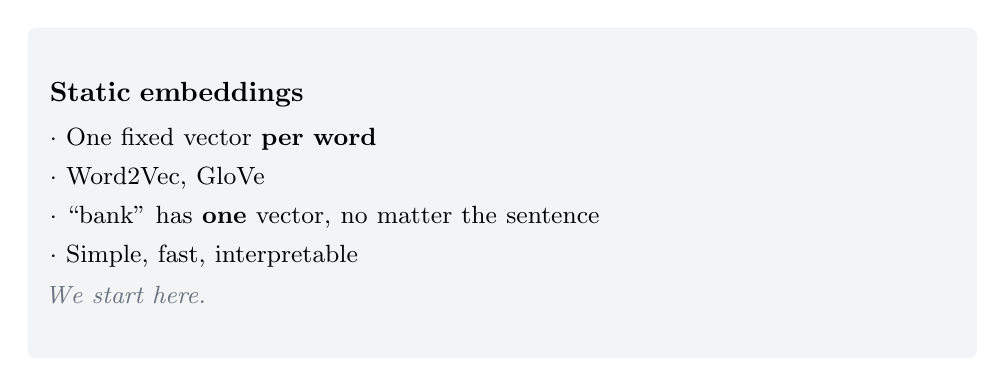
\begin{tikzpicture}
    \node[fill=lightgray, rounded corners=3pt,
          inner xsep=8pt, inner ysep=8pt, text width=\columnwidth-18pt, minimum height=4.2cm]{%
      \textbf{Static embeddings}\\[5pt]
      {\small
      $\cdot$ One fixed vector \textbf{per word}\\[3pt]
      $\cdot$ Word2Vec, GloVe\\[3pt]
      $\cdot$ ``bank'' has \textbf{one} vector, no matter the sentence\\[3pt]
      $\cdot$ Simple, fast, interpretable\\[3pt]
      \textcolor{midgray}{\textit{We start here.}}}};
  \end{tikzpicture}

  \column{0.48\textwidth}
  \vspace{0pt}
  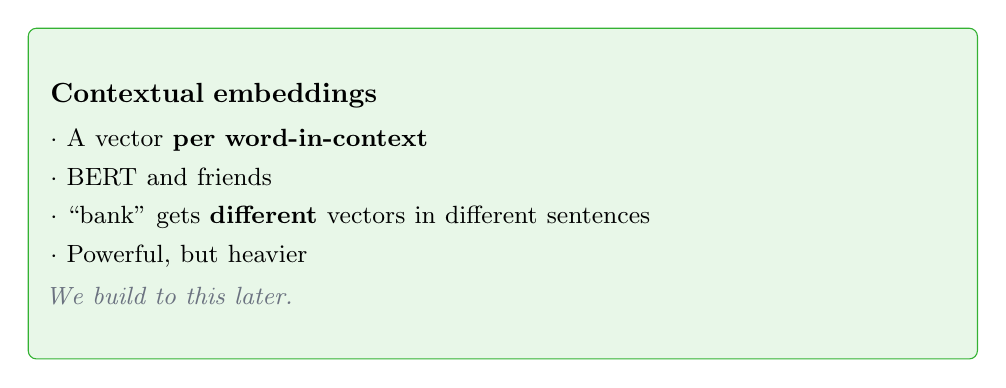
\begin{tikzpicture}
    \node[fill=lightgreen, draw=wurgreen, rounded corners=3pt,
          inner xsep=8pt, inner ysep=8pt, text width=\columnwidth-18pt, minimum height=4.2cm]{%
      \textbf{Contextual embeddings}\\[5pt]
      {\small
      $\cdot$ A vector \textbf{per word-in-context}\\[3pt]
      $\cdot$ BERT and friends\\[3pt]
      $\cdot$ ``bank'' gets \textbf{different} vectors in different sentences\\[3pt]
      $\cdot$ Powerful, but heavier\\[3pt]
      \textcolor{midgray}{\textit{We build to this later.}}}};
  \end{tikzpicture}
\end{columns}

\medskip
{\small\textcolor{midgray}{\textit{Both rest on the same foundation: meaning from context.
The difference is whether context is baked in once, or computed fresh each time.}}}
\end{frame}

% ── SLIDE 10: Recap ──────────────────────────────────────────────────────────
\begin{frame}{Foundations: The Takeaways}
\vspace{0.3cm}
\begin{itemize}\setlength\itemsep{9pt}
  \item[\textcolor{wurgreen}{\faCheck}]
    Bag-of-words fails because it treats words as \textbf{isolated symbols}
  \item[\textcolor{wurgreen}{\faCheck}]
    The \textbf{distributional hypothesis}: a word's meaning can be inferred from the
    \textbf{contexts it appears in}
  \item[\textcolor{wurgreen}{\faCheck}]
    \textbf{Embeddings} represent each word as a \textbf{dense vector} in a shared
    meaning-space
  \item[\textcolor{wurgreen}{\faCheck}]
    In that space, \textbf{distance} reflects similarity and \textbf{directions} can carry
    meaning (analogies)
  \item[\textcolor{wurgreen}{\faCheck}]
    Two flavors: \textbf{static} (one vector per word) and \textbf{contextual}
    (one vector per use)
\end{itemize}

\medskip
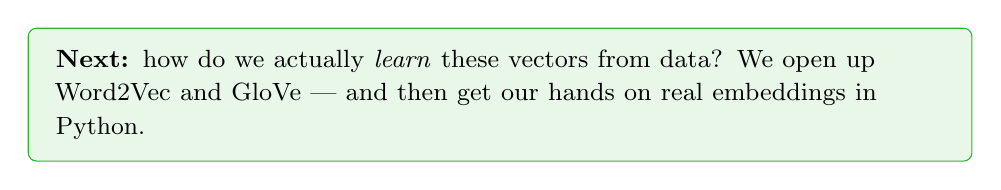
\begin{tikzpicture}
  \node[fill=lightgreen, draw=wurgreen, rounded corners=3pt,
        inner xsep=10pt, inner ysep=8pt, text width=\textwidth-24pt]{%
    {\small\textbf{Next:} how do we actually \emph{learn} these vectors from data?
    We open up Word2Vec and GloVe --- and then get our hands on real embeddings in Python.}};
\end{tikzpicture}
\end{frame}

\end{document}
